          \section{Modelle}
Im folgenden Teil werden die entwickelten Deep Learning Modelle vorgestellt. Für jedes Modell ist der grundlegende Ablauf derselbe (siehe Abbildung \ref{img:workflow}). Die Aufnahme wird vorab auf die Länge 5s zugeschnitten. Anschliessend wird ein Spektrogramm generiert. Die Werte des Spektrogramms werden in die Dezibell Skala umgerechnet und dann normiert. Die Grösse des Spektrogramms unterscheidet sich zwischen den Modellen. Schliesslich berechnet ein Neuronales Netzwerk aus dem Spektogramm eine Vorhersage für die drei Sprachen. 
\\
Insgesamt werden drei grundsätzlich verschiedene Neuronalen Netzwerk Architekturen vorgestellt. Die ersten zwei Modelle sind Convolutional Neural Networks während das dritte Modell eine Kombination zwischen CNN und Recurrent Neural Network ist. Jedes Modell endet mit einer Ausgabeschicht der Grösse drei. Jeder der der drei Werte steht für die Wahrscheinlichkeit einer Sprache. Um zu garantieren, dass die Summe der Werte 1 gibt wird die Aktivierungsfunktion \textit{softmax} verwendet:
$$ \text{softmax}(\boldsymbol x)_i = \frac{\text{exp}(x_i)}{\sum_{j=0}^{n} \text{exp}(x_j)}$$
Beispiel: 
$$ \text{softmax}(\begin{bmatrix} 0.5 & 0.8 & 0.3\end{bmatrix}) = \begin{bmatrix} 0.31 & 0.43 & 0.26\end{bmatrix} = \begin{bmatrix} p_{FR} & p_{EN} & p_{DE}\end{bmatrix}$$
Die Funktion eignet sich generell für Klassifizierung, denn sie bildet die Werte auf eine Wahrscheinlichkeitsverteilung über die berechneten Ausgabeklassen ab \parencite[][S. 180-184]{goodfellow}. Der Wert einer Ausgabeklasse lässt sich auf diese Weise als die Wahrscheinlichkeit $p_{X}$ interpretieren: Die Wahrscheinlichkeit, dass die Eingabe in der Sprache X ist. Für alle anderen Schichten wird immer die Aktivierungsfunktion \textit{ReLU} verwendet.
\\
Damit die Ziele des Netzwerks die gleichen Anzahl Dimensionen wie die Ausgaben haben, werden sie \textit{One-hot}\parencite{chollet} kodiert. Das bedeutet, dass die richtige Sprache die Wahrscheinlichkeit 1.0 besitzt und alle anderen 0. Das Ziel für eine französische Aufnahme ist also $\begin{bmatrix} 1.0 & 0.0 & 0.0\end{bmatrix}$, für eine englische Aufnahme $\begin{bmatrix} 0.0 & 1.0 & 0.0\end{bmatrix}$, etc.. Obwohl die Ziele die gleiche Form wie die Ausgaben haben lässt sich der Verlustwert nicht so leicht berechnen wie beim Anfangsbeispiel. Die standard Verlustfunktion in diesem Fall ist \textit{Categorical Crossentropy}\parencite{chollet}. Für das Ziel $\boldsymbol{p} \in \mathbb{R}^n$ und die Voraussage $\boldsymbol{\hat{p}} \in \mathbb{R}^n$ ist die Funktion folgendermassen definiert:

$$H(\boldsymbol{p}, \hat{\boldsymbol{p}}) = -\sum\limits_{i} p_i \cdot \log \hat{p_i}$$
\\
Dass diese Verlustfunktion sinnvoll ist, lässt sich intuitiv verstehen: Das Ziel des Netzes soll es sein, die Wahrscheinlichkeit der richtigen Sprache zu maximieren. So soll zum Beispiel bei $\boldsymbol{p}=\begin{bmatrix} 0 & 1.0 & 0\end{bmatrix}$ und $\boldsymbol{\hat{p}}=\begin{bmatrix} p_0 & p_1 & p_2\end{bmatrix}$,  $ p_1$ maximiert werden. Die Wahrscheinlichkeit der richtigen Sprache lässt sich einfach berechnen:
$$L(\boldsymbol{p}, \hat{\boldsymbol{p}}) = \sum\limits_{i} p_i \cdot \hat{p_i}$$
Im Beispiel oben fallen $P_0$ und $P_2$ weg und $1\cdot P_1$ bleibt übrig, was genau der Wahrscheinlichkeit der richtigen Sprache entspricht. Ab hier lässt sich nachvollziehen, das genau wie wir $L$ maximieren wollen, $-L$ (wie der Verlustwert) minimiert werden soll. Da $\text{log}$ eine monoton steigende Funktion ist, ist $f(x)$ an der gleichen Stelle minimal wie $f(\log x)$. Was folgt ist genau die Categorical Crossentropy. Kurzgesagt sind die Parameter des Netzwerk die selben wenn $H$ minimiert oder $L$ maximiert wird: \parencite[vgl. ][]{entropy}
\begin{align*}
\shortintertext{Sei $X\in \mathbb{R}^n$ alle Parameter des Netzwerks so dass}
   L(\boldsymbol{p}(X), \boldsymbol{\hat{p}}) &= \max\limits_x\{L(\boldsymbol{p}(x), \boldsymbol{\hat{p}})\}
\shortintertext{folgt, dass}
-L(\boldsymbol{p}(X), \boldsymbol{\hat{p}}) &= \min\limits_x\{-L(\boldsymbol{p}(x), \boldsymbol{\hat{p}})\}
\shortintertext{und daraus folgt, dass}
-L(\boldsymbol{p}(X), \log\boldsymbol{\hat{p}}) &= \min\limits_x\{-L(\boldsymbol{p}(x), \log\boldsymbol{\hat{p}})\}\\
H(\boldsymbol{p}(X), \boldsymbol{\hat{p}}) &= \min\limits_x\{H(\boldsymbol{p}(x), \boldsymbol{\hat{p}})\}
\end{align*} 


Die Hyperparameter der Modelle, wie zum Beispiel die Grösse des Spektrogramms wurden empirisch bestimmt. Insgesamt wurden fast 200 Experimente durchgeführt. Allerdings konnte längst nicht jede mögliche Kombination von Hyperparametern probiert werden, da jeder Durchlauf zeitaufwändig und nicht parallelisierbar ist.
\begin{figure}[hbt]
	\centering
		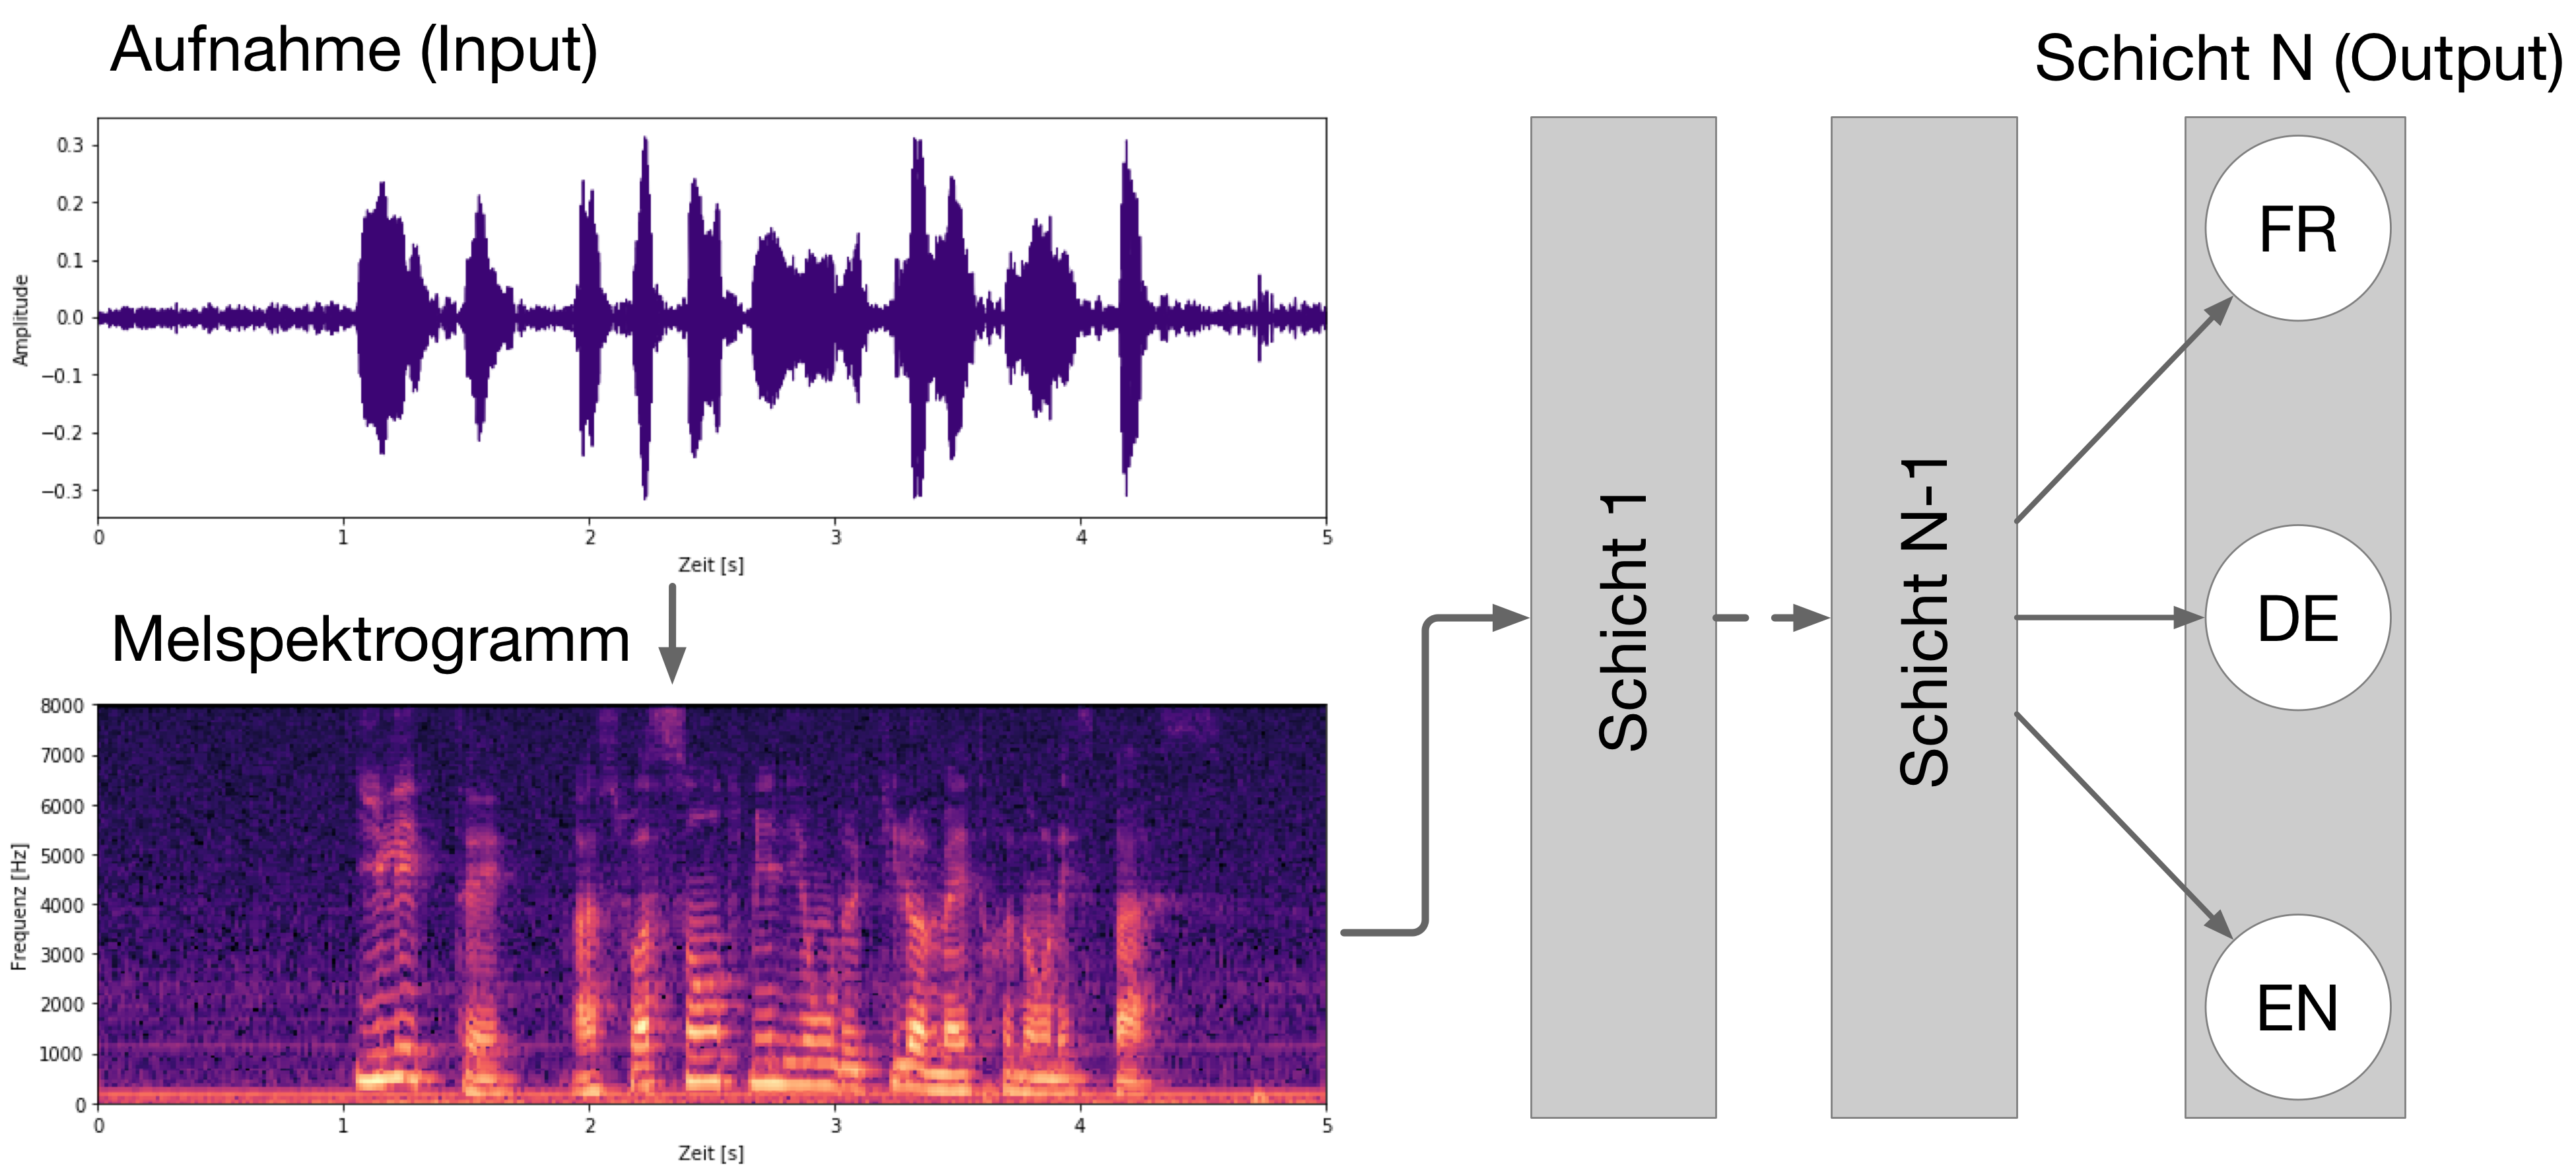
\includegraphics[width=0.8\textwidth]{assets/modelflow.png}
	\caption{Grundlegender Aufbau aller Modelle}
	\label{img:workflow}
\end{figure}


\subsection{CNN}
Das CNN Netzwerk akzeptiert Spektrogramme der Grösse 28x313, wobei 28 verschiedene Mel-Frequenzeimer berechnet werden an 313 Zeitpunkten. Das Netz besteht aus drei Convolution-MaxPooling Blocks und zwei Dense Schichten (Abbildung \ref{img:cnn}). Die Convolution-Grösse ist immer 3x3 und MaxPooling geschieht im Bereich 2x2. Die Anzahl Convolution's (Kanäle) nimmt von 64 auf 128 zu. 
\\
Die \textit{Fully Connected} Schicht besteht aus 512 Knoten mit 30\% \textit{Dropout}. Bei Dropout wird ein zufälliger gewählter Anteil der Eingabe der Schicht mit 0 ersetzt. Das Netz lernt dann, ohne diese Verbindungen auszukommen und somit mehrere Verbindungen einzelnen starken Verbindungen vorzuziehen. Die Eigenschaft hat einen positiven Einfluss auf die Robustheit des Netzes gegenüber neuen Daten \parencite[][Kap. 4.4.3]{chollet}.
\\
Die Architektur entspricht massgeblich der vorgestellten Architektur in \parencite{iLID} plus Dropout.
 \begin{figure}[hbt]
	\centering
		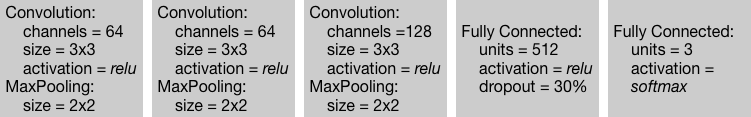
\includegraphics[width=0.8\textwidth]{assets/cnn.png}
	\caption{CNN Architektur}
	\label{img:cnn}
\end{figure}

\subsection{MobileNet-CNN}
Andere Arbeiten hatten gezeigt, dass grosse CNN Architekturen die auf dem \textit{ImageNet}\parencite{imagenet} Datenset (Riesiges Bilddatenset mit tausenden Bidklassen) stark sind, ebenfalls für Audioklassifizierung geignet sind \parencite{cnn_large}. Um Leistung zu sparen wurden Experimente mit \textit{MobileNet} durchgeführt.
MobileNet ist eine bekannte CNN Architektur entwickelt von \textit{Google} \parencite[][(V2)]{mobilenet}. Das Modell ist speziell entwickelt für Mobilgeräte, die in der Regel schwächere Hardware als Desktop-Computer besitzen. Das Ziel war ein effizientes Netzwerk für Bilderkennung im grossen Umfang, wie z.B ImageNet. Da das Modell in dieser Arbeit nur zwischen drei Klassen unterscheiden muss, wird die Anzahl Knoten im Netzwerk so weit wie möglich verkleinert, bzw. der Parameter $\alpha$ im Paper wird auf 0.25 gesetzt. 
\\
Das Netzwerk besitzt insgesamt 21 Schichten. Das Netzt funktioniert am bessten mit Eingaben der Grösse 224x224, der Bildgrösse in ImageNet. Die Spektrogramme werden darum auf dieses Format skaliert.
 \begin{figure}[hbt]
	\centering
		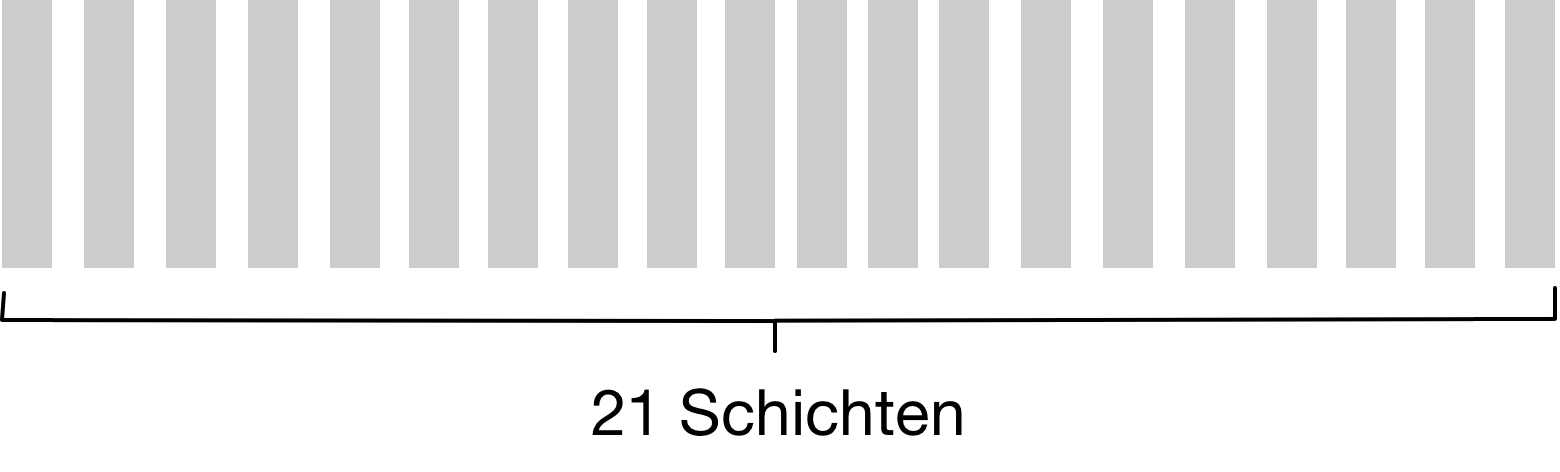
\includegraphics[width=0.8\textwidth]{assets/mobilenet.png}
	\caption{MobileNet Architektur}
	\label{img:mobilenet}
\end{figure}

\subsection{CRNN}
Convolutional Recurrent Neural Networks, eine Mischung aus CNN und RNN, wurden bereits erfolgreich auf Sprachidentifikation angewendet \parencite{crnn}\parencite{yerevann}. RNN's für Tonaufnahmen zu verwenden ist sinnvoll, denn Audiodaten sind naturgemäss zeitliche Folgen, also ideal für RNN's. RNN's haben aber den Nachteil, dass sie langsam lernen. Darum soll der CNN Teil im Vorfeld aus dem Spektrogramm eine kompaktere Repräsentation berechnet, z.b eine Abfolge von Phonemen. Da die Lernzeit proportional zur Eingabegrösse ist, lernt der RNN teil mit dieser Eingabe schneller. Es gibt keine Möglichkeit zu verifizieren, ob das CNN wirklich Phoneme berechnet aber die Resultate zeigen, dass das CRNN besser abschneidet als das CNN.
\\
Der CNN Teil besteht aus fünf Blocks von Convolution, MaxPooling und \textit{Batch Normalization}\label{Batch Normalization} (Siehe Abbildung \ref{img:crnn}). Die Idee von \textit{Batch Normalization} ist, dass die Ausgabe der vorherigen Schicht so normalisiert wird, dass sie den Durchschnitt 0 und die Varianz 1 besitzt. \textit{Batch Normalization} bringt den vor allem den Vorteil, dass das Modell schneller konvergiert, also schneller bessere Leistungen erbringt. \parencite{batch}
\\
Die Anzahl Convolutions steigert sich schrittweise von 16 auf 64. Das Convolution-Fenster hat immer die Grösse 4x4 und MaxPooling das Fenster 2x2. Bei den Convolutions wird 0.01 \textit{L2-Regularisation} verwendet:
$$ Verlust = Verlust + \sum_{i} w_{i}^{2}$$
Das bedeutet, dass dem Verlustwert zusätzlich das Quadrat der Gewichte addiert wird \parencite[Kap.~7.1.1]{goodfellow}. Übermässig hohe Gewichte werden überproportial gewertet. Die Regularisation hat das gleiche Ziel wie Dropout, das Netz robuster zu gestalten.
\\

 \begin{figure}[hbt]
	\centering
		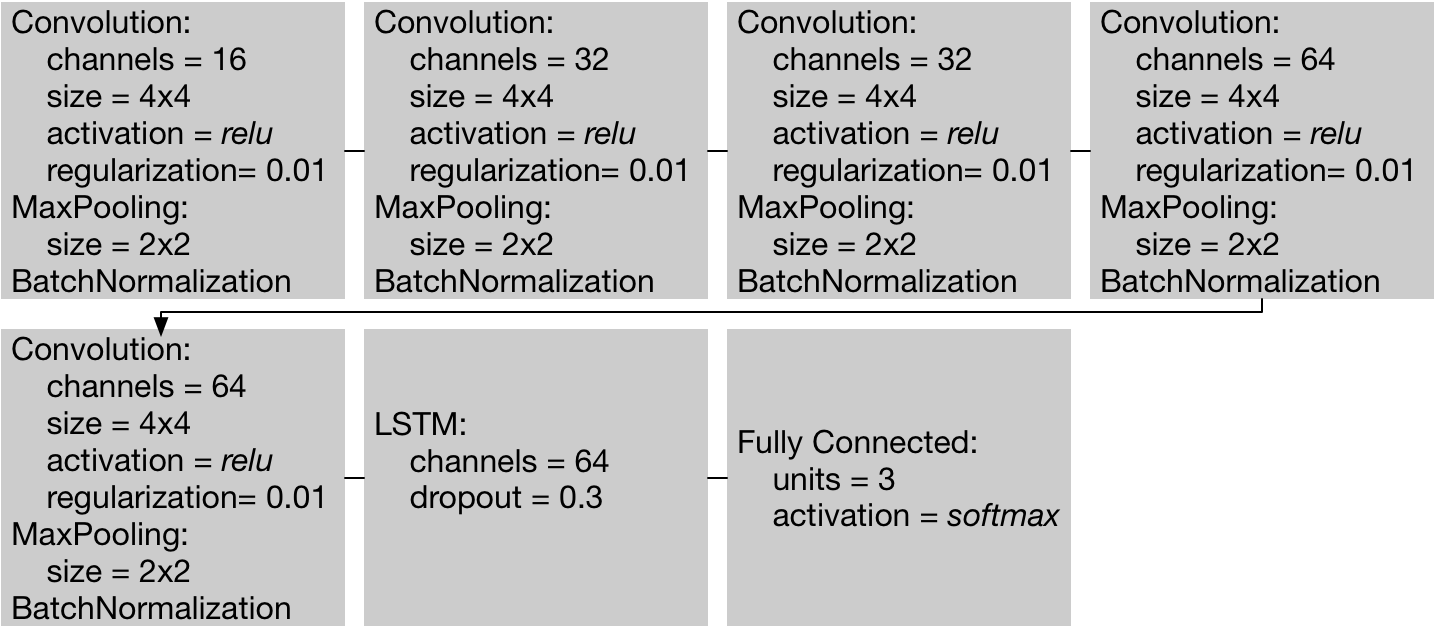
\includegraphics[width=0.8\textwidth]{assets/crnn.png}
	\caption{CRNN Architektur}
	\label{img:crnn}
\end{figure}

\section{Umsetzung und Resultate}

\subsection{Implementierung}

Was in dieser Arbeit theoretisch gemacht wurde, wurde bis hierhin ausführlich beschrieben. Die praktische Implementierung aller Schritte wurde aber noch nicht behandelt. Dieses Kapitel erklärt die genaue Umsetzung aller Teile und nennt die verwendeten Werkzeuge. In anderen Worten wird hier die praktische Arbeit anschaulich gemacht.
Für alle Teile der Arbeit wird mir der Programmiersprache \textit{Python}  gearbeitet. Python eignet sich generell für Deep Learning weil viele Bibliotheken für die Sprache geschrieben sind. Ausserdem hat Python den Vorteil, dass es einsteigerfreundlich ist. Python kann entweder als Script geschrieben werden, also als Datei die ausgeführt wird, oder in einem interaktiven \textit{Jupyter Notebook}\parencite{jupyter}. Jupyter Notebook's  bestehen unter anderem aus mehreren Textzellen die einzeln ausgeführt werden können aber den gleichen Thread teilen. Das macht Jupyter Notebooks unglaublich praktisch für das Experimentieren und Darstellen von Daten.
\\ \\
Die Aufgabe lässt sich in vier Teile gliedern. Abbildung \ref{img:vorgehen} zeigt die Teile schematisch. 
Als erstes müssen die zu verwendeten Daten aus den verschiedenen Quellen gesammelt werden. Bevor die Daten aber heruntergeladen werden muss in manchen Fällen eine Selektion geschehen. So kann bei Youtube aufgrund der riesigen Anzahl an verfügbaren Videos unmöglich die gesamte Datenmenge gesammelt werden. Aus diesem Grund wurde bei Youtube manuell nach geeigneten Kanälen bzw. Playlists gesucht. Nach dem klar ist was gesammelt werden soll kann man mit dem Herunterladen starten. Dafür werden Python-Scripts geschrieben die die beträchtliche Menge Daten automatisiert herunterladen. Für die YouTube Daten wird die externe Bibliothek \textit{Youtube-dl}\parencite{youtube-dl} benutzt.

 \begin{figure}[hbt]
	\centering
		
\includegraphics[width=1.0\textwidth]{assets/vorgang_small.png}
	\caption{Überblick über die Arbeitsschritte}
	\label{img:vorgehen}
\end{figure}

Der zweite Schritt ist das Erforschen der Daten. Darunter wird zum Beispiel das herausarbeiten von wichtigen Unterschieden zwischen den Datenquellen verstanden. Unter anderem wurde in diesem Schritt eine einheitliche Länge und Abtastrate der Aufnahmen festgelegt. Für diesen Teil sind Jupyter Notebook's ideal.  Für das einlesen der Audiodaten wird die Bibliothek \textit{Librosa}\parencite{librosa} verwendet und alfällige Grafiken werden mit der Bibliothek \textit{Matplotlib}\parencite{matplotlib} erstellt.
\\
Als nächstes können die Daten korrekt strukturiert werden. Das heisst das die Daten einerseits in Training, Validation und Testdaten gespalten werden während sie gleichzeitig nach der Sprache geordnet sind. Vor dem definitiven abspeichern der Daten werden sie auch auf die richtige Länge zugeschnitten. Das Format der Daten ist ein \textit{Numpy}-Array\parencite{numpy}. Numpy stellt praktische Funktionen für numerische Operationen bereit und kann die Daten effizient abspeichern. Programmiert wird dieser Teil in einer Mischung aus Python-Scripts und Jupyter Notebook's.
\\
Zum Schluss kommt Machine Learning ins Spiel. Der letze Schritt ist das Experimentieren mit unterschiedlichen Modellen. Erst jetzt werden Netzwerke trainiert und ausgewertet. Die zwei wichtigen Bibliotheken für den Machine Learning Teil sind \textit{Keras}\parencite{keras} und \textit{Tensorflow}\parencite{tensorflow}. Tensorflow ist die Machine Learning Bibliothek von Google. Dank Tensorflow müssen keine neuronalen Netze von Grund auf programmiert werden. Tensorflow übernimmt alle Arbeit ausser das tunen von Hyperparametern. Keras ist lediglich ein einfaches Interface für Tensorflow und andere Machine Learning Bibliotheken. Der Code für das Trainieren eines einfachen Keras Modells findet sich im Anhang. 


\subsection{Auswertung an Voxforge und YouTube}

An dieser Stelle werden die drei Modelle ausgewertet. Es wird gemessen wie gut die Modelle Aufnahmen klassifizieren. Die verwendete Messgrösse um die Modelle zu vergleichen ist die Genauigkeit. Die Genauigkeit beschreibt den Anteil an richtig klassifizierten Aufnahmen:
$$Genauigkeit = \frac{\# \text{ Korrekt klassifizierte Aufnahmen}}{\# \text{ Total Aufnahmen}}$$
Genauigkeit ist in diesem Fall eine angebrachte Messgrösse, weil die Daten gleichmässig über die Sprachen verteilt sind. Ist dies nicht der Fall kann die Genauigkeit täuschen. Wenn zum Beispiel 90\% der Daten Deutsch wären, würde hypothetisch ein Modell dass immer Deutsch ausgiebt 90\% Genauigkeit haben. Obwohl das hypothetische Modell extrem naiv ist, täuscht die hohe Genauigkeit. Im Fall dieser Arbeit wurde darum ausdrücklich auf eine gleichmässige Verteilung der Daten geachtet.
\\ 
Die Modelle werden separat an allen drei Datenquellen ausgewertet. Für jedes Datenset wurden alle Modelle drei Mal trainiert. Die schlussendliche Genauigkeit ist die beste der drei Versuchen. Die Genauigkeiten am Voxforge Testset sind in Tabelle \ref{table:test_vox} geschrieben.
\begin{table}[h]
	\centering
	\begin{tabular}{llll}
		\hline
		Netz & Architektur     & Genauigkeit \\ \hline
		CNN  & 3 Conv          & 95.5\%      \\
		CRNN & 4 Conv + GRU   & 96.9\%       \\
		MobileNet  & 28 Conv + Dense & 86.1\%       \\ \hline
	\end{tabular} \\
	\caption{Beste Voxforge Genauigkeit}
	\label{table:test_vox}
\end{table}
Das CRNN führt mit fast 97\%, dicht gefolgt vom CNN. Das MobileNet besitzt eine mehr als 10\% tiefere Genauigkeit. Obwohl der Unterschied zwischen CRNN und CNN absolut klein erscheint, ist er relativ zum Fehler beträchtlich. Das CRNN hat eine mehr als 30\% kleinere Fehlgenauigkeit als das CNN.
\\ 
Die Genauigkeiten am Youtube Testset zeigt Tabelle \ref{table:test_you}. Sämtliche Modelle haben am Youtube Testset eine tiefere Genauigkeit als am Voxforge Testset. Das MobileNet vollzieht mit einem Verlust von 5.9\% Genauigkeit den grössten Fall. Das CNN und CRNN besitzen beide eine Genauigkeit von 94.7\%.
\\
Die bisherigen Resultate zeigen, dass das CRNN insgesamt die höchste Genauigkeit hat. Trotzdem heisst das nicht, dass das CRNN in jedem Fall besser ist als die anderen beiden Modelle. Der Beweis dafür ist, dass eine Kombination aller Modelle oft besser ist, als die einzelnen Modelle. Ein Modell berechnet aus dem Durchschnitt der drei Modelle erreicht bei Voxforge eine Genauigkeit von 97.9\%. Das bedeutet eine erneute Verkleinerung der Fehlgenauigkeit um mehr als 30\%.
\begin{table}[h]
	\centering
	\begin{tabular}{llll}
		\hline
		Netz & Architektur     & Genauigkeit  \\ \hline
		CNN  & 3 Conv          & 94.7\%       \\
		CRNN & 4 Conv + LSTM   & 94.7\%     \\
		MobileNet  & 28 Conv + Dense & 80.2\%   \\ \hline
	\end{tabular}
	\caption{Beste YouTube Genauigkeit}
	\label{table:test_you}
\end{table}
\\
Das CRNN hat die höchste einzelne Genauigkeit zum Preis einer langen Trainingsdauer. Das CRNN braucht mehr als drei mal so lang zum trainieren wie das CNN. Das Genauigkeit/Zeit Verhältnis des CNN ist bedeutend grösser als das des CRNN. Die Trainingszeiten sind in Tabelle \ref{table:test_time} aufgetragen.
\begin{table}[h]
	\centering
	\begin{tabular}{lll}
		\hline
		Netz & Trainingsdauer \\ \hline
		CNN  & 20 min \\
		CRNN & 70 min \\
		MobileNet  & 60 min\\ \hline
	\end{tabular}
	\caption{Trainingsdauer}
	\label{table:test_time}
\end{table}
\\
Eine weitere Methode um neben der Genauigkeit die Modelle auszuwerten, ist eine Wahrheitsmatrix aufzustellen. Die Zeilen der Matrix entsprechen der Sprache der Aufnahmen, während die Spalten die berechnete Antwort des Algorithmus unterscheiden. Das Feld oben links zeigt zum Beispiel die Anzahl der französischen Aufnahmen die als Französisch klassifiziert wurden. Die Wahrheitsmatrix gibt zeigt somit mehr Details als die Genauigkeit alleine. Abbildung \ref{img:matrix_vox} zeigt die Matrix vom CRNN Modell an den kombinierten Testdaten von Youtube und Voxforge.
\\
Das interessante das an dieser Matrix ablesbar ist, ist dass das Modell Englisch und Deutsch relativ oft verwechselt: Englisch wird in 121 Fällen mit Deutsch verwechselt und Deutsch wird 122 mal dem Englischen verwechselt. Im Vergleich werden Französisch und Deutsch insgesamt nur in 67 Fällen verwechselt. Französisch und Englisch werden insgesamt 105 mal verwechselt.
 \begin{figure}[hbt]
	\centering
		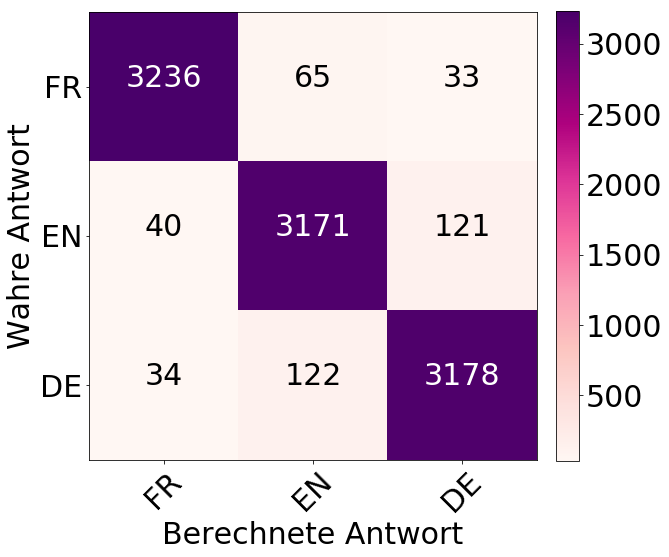
\includegraphics[width=0.5\textwidth]{assets/matrix_voxyou_crnn.png}
	\caption{Wahrheitsmatrix von CRNN an Voxforge und Youtube (Total 10'000 Aufnahmen)}
	\label{img:matrix_vox}
\end{figure}

\subsection{Auswertung an Librivox}
Die Genauigkeit bei den Voxforge und Youtube Daten war sehr hoch, weil die Modelle die beiden Quellen bereits kannten. Obwohl das Testset unterschiedlich vom Trainingsset ist,  teilen sie viele Gemeinsamkeiten. Die Librivox Daten sind den Modellen hingegen komplett fremd. Mit der Auswertung an den Librivox Daten wird klar, wie gut das Modell generalisiert, bzw. wie gross die Stichprobenverzerrung ist.
\\
Tabelle \ref{table:test_lib} zeigt die Genauigkeiten auf dem Librivox Testset. Das CNN verliert im Vergleich zu vorher rund 6\% Genauigkeit. Das CRNN hingegen erreicht immer noch 94.1\% Genauigkeit. Am schlimmsten geht es dem MobileNet, das auf eine Genauigkeit von 56.8\% sinkt. Anhand dieses Verlust lässt sich klar ablesen, dass das MobileNet sich an die Trainingsdaten überangepasst hat. Das CRNN und CNN auf der anderen Seite generalisieren überraschend gut.
\begin{table}[h]
	\centering
	\begin{tabular}{llll}
		\hline
		Netz & Architektur     & Genauigkeit  \\ \hline
		CNN  & 3 Conv          & 88.1\%       \\
		CRNN & 4 Conv + LSTM   & 94.1\%       \\
		MobileNet  & 28 Conv + Dense & 56.8\%       \\ \hline
	\end{tabular}
	\caption{Beste Librivox Genauigkeit}
	\label{table:test_lib}
\end{table}
\\
Genau wie bei Voxforge und Youtube lässt sich wieder eine Wahrheitsmatrix zu detaillierten Auswertung erstellen. Abbilung \ref{img:matrix_lib} zeigt die Matrix des CRNN Modells. Auffällig an dieser Matrix ist, dass Englisch relativ selten mit anderen Sprachen verwechselt wird. Deutsch und Französisch werden hingegen oft fälschlicherweise als Englisch erkannt. 
\begin{figure}[hbt]
	\centering
		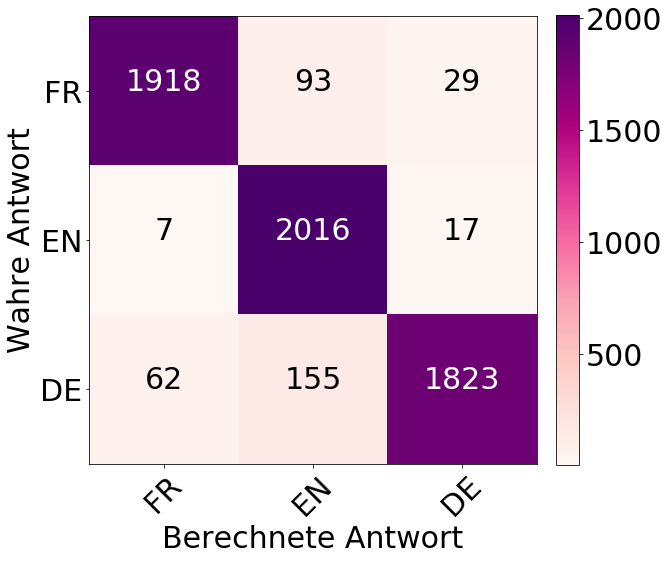
\includegraphics[width=0.5\textwidth]{assets/matrix_lib_crnn.png}
	\caption{Wahrheitsmatrix von CRNN an Librivox (Total 6120 Aufnahmen)}
	\label{img:matrix_lib}
\end{figure}
